%!TEX root = index.tex

\section{Air Traffic Control}

The main objective of Air Traffic Control is to prevent collisions between aircraft in air or on the ground and to expedite the flow of air traffic. \cite[Chapter 2.2]{annex11} In order to do so effectively, the airspace is divided to separate areas which are controlled by different ATC services depending on their characteristics.

\subsection{Air Traffic Control Services}

ATC services can be divided into Area Control Service (ACC), Approach Control Service (APP) and Aerodrome Control Service (TWR) \cite[Chapter 1]{doc4444} 

The airspace in which ATC service is provided can be divided into Control Area (CTA) and Control Zones (CTR). Within CTA, Terminal Control Areas (TMA) are established to help in arrival and departure at some airports.

Control Zones are normally situated below CTA and encompass airspace used by flights arriving at and departing from aerodromes. CTR extends from the ground at least to the lower limit of CTA, but may extend further. CTR may include several aerodromes situated close together. \cite[Chapter 2.10]{annex11} The Figure \ref{fig:airspace} shows how the controlled airspace can be divided and which services provide control in which areas.

\begin{figure}[h]
    \centering
    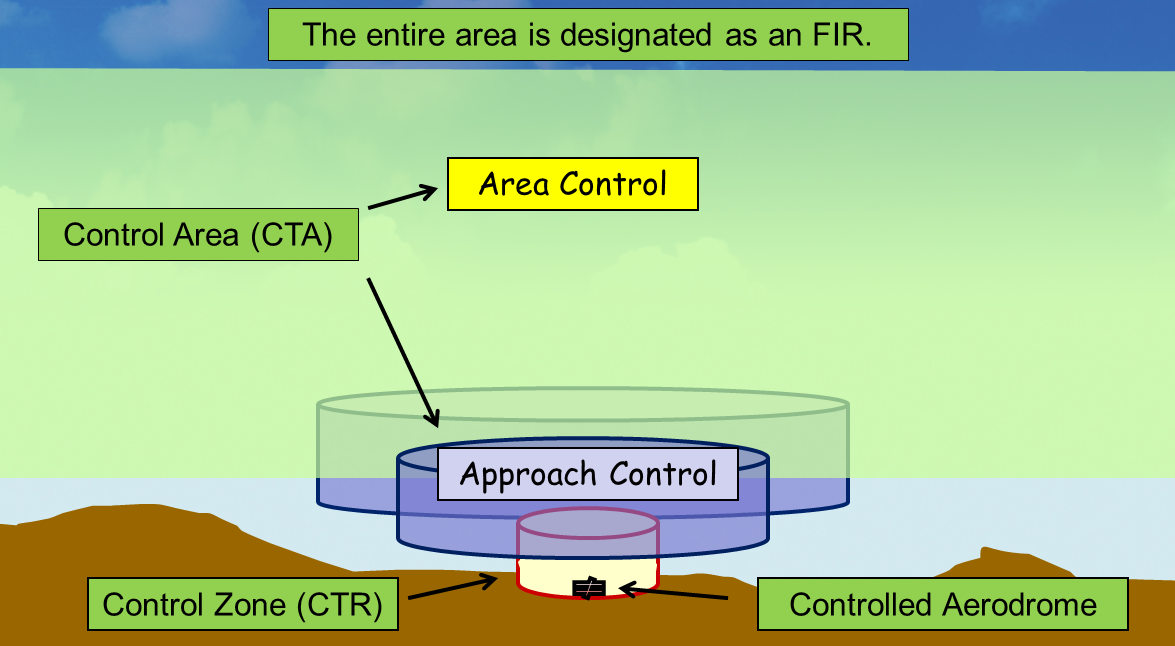
\includegraphics[width=0.9\textwidth]{figures/airspace.png}
    \caption{Airspace division and control \cite[Chapter 2.10]{annex11}}
    \label{fig:airspace}
\end{figure}

\subsubsection{Area Control Service}

Area Control Service is an ATC service provided by Area Control Center responsible for flights in Control Areas (CTA). Normally ACC is identified by the name of a nearby city, area or landmark. Smaller countries usually have one ACC, but many larger countries are controlled by several. ACCs usually control aircraft in their en-route phase of flight. The ACC may be also responsible for flights to and from smaller aerodromes with no separate approach control service. \cite[Chapter 3.2]{annex11}

Control Area contains airways, Terminal Control Areas (TMA) and other airspace. It extends upwards from specified altitude.

\subsubsection{Approach Control Service}

Approach Control Service (APP) is ATC service that is responsible for the part of CTA and CTR required by arriving or departing controlled flights. This area is called Terminal Control Area (TMA or TCA) in U.S. or Terminal Manoeuvring Area (TMA) in Europe. The primary functions of APP is sequencing arriving aircraft and assisting departing aircraft in becoming established on course. The arrival and departure functions can be divided into several positions on busy aerodromes. APP is usually identified by the name of the aerodrome which it is serving, but sometimes it's not collocated with TWR and is at distant ACC location away from the airport it serves. When no separate APP exists, approach control service is provided by ACC or TWR. \cite[Chapter 3.2]{annex11}

\subsubsection{Aerodrome Control Service}

Aerodrome Control Service is provided by a control tower (TWR) and is responsible for aircraft landing and taking off. It's also responsible for planes flying under Visual Flight Rules (VFR) in the CTR and for preventing collisions between aircraft on the manoeuvring area of the aerodrome. \cite[Chapter 3.2]{annex11}

\subsection{Coordination within ATC}

The airspace in CTA is further divided to sectors to allow for effective control. The shape and size of the sectors is determined by usual traffic going through them. Near busy aerodromes lay smaller sectors and larger sectors are located in higher altitude or places with low traffic like Alaska.

TMA airspace isn't further divided, but rather controlled by single sector. TWR controlled airspace is located inside CTR sector. 

The sectors are grouped within Air Route Traffic Control Centers. Each center has its  controller who provides high-level view on the air traffic flow and manages overall traffic flow especially in cases like approaching storms that require traffic flow to be diverted across several sectors.

The coordination can take place between ATC centers, between ACC and APP, APP and TWR and between individual sectors inside ACC. The coordination between ATC sectors is usually conducted in relation to transfer of control of individual flights or while planing the air traffic flow. The detailed rules and procedures of the communication are often defined in local Letter Of Agreement (LOA) between the sectors.

\subsubsection{Transfer of Control Between Sectors}

Every flight must be controlled by single ATC unit at any time. When the flight plan of an aircraft crosses several sectors, they must transfer the responsibility for the flight along the way. The transfer of control must be approved by the accepting sector and the point of transfer agreed by both units.

The transfer can be divided into three stages: first the pilot is notified to prepare to change sectors, then the conditions of the transfer are negotiated and finally after agreeing the control is transferred to the accepting sector. This process can be achieved by automated means without the need of traditional telephone coordination between the sectors. \cite[Chapter 10]{doc4444}

\subsubsection{Coordination between ACC and APP}

After ACC releases a flight to APP, APP may apply clearances to the aircraft without reference to ACC. In case of missed approach, ACC is informed as soon as possible if aircraft will fly back to CTA.

The take-off time is specified by APP with respect to traffic in the TMA sector. The take-off time can be also specified by ACC in case it needs to coordinate the departure flow with other ACC traffic. APP and ACC can also agree on expiry time for departure clearance if delay of take-off would cause separation problems.

APP keeps ACC informed about used runway and type of instrument approach procedure, minimal time between successive arrivals, revision of estimated arrival times for transferring flights, departure times, missed approach times and other information about controlled traffic that may affect ACC. ACC informs APP about identification, type and point of transfer of incoming aircraft, anticipated delay to departures because of congestion and other information agreed on by both parties.\cite[Chapter 10]{doc4444}

\section{Airspace Classes}

The controlled airspace can be also classified in one of the Classes A-G. The classification is mutually exclusive so Class A airspace can't be also classified as Class D at the same time and in the same place. The classes define the flight rules used in the airspace, interactions between pilot and Air Traffic Control and most importantly the responsibility for avoiding other aircraft which can be assigned either to the ATC or to the pilot himself. \cite{annex11}

The definition of the classes is given by ICAO and is respected by most countries although some differences in the specification can exist. The use of the classes is nation specific, some countries classify their whole airspace into just one or few classes, some use all classes. Which classes are used in which parts of the airspace also varies greatly. \cite{classes} The typical use of airspace classes in USA can be seen in Figure \ref{fig:classes}.

\begin{figure}[h]
    \centering
    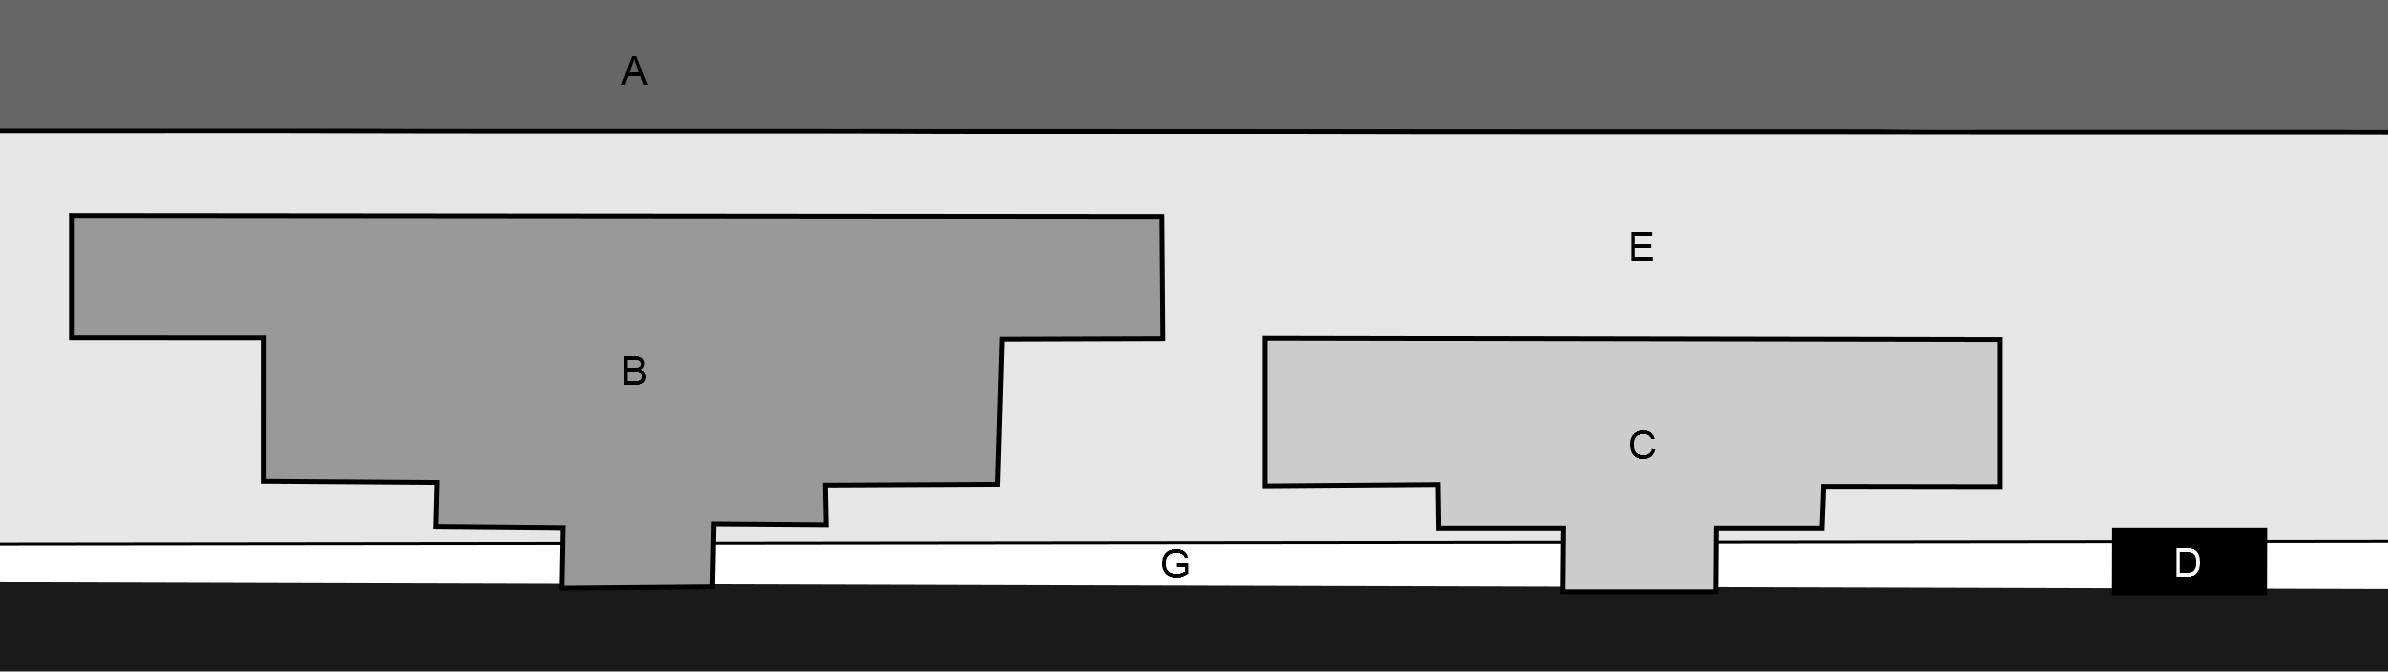
\includegraphics[width=\textwidth]{figures/classes.png}
    \caption{Airspace Classification Example \cite{nolan}}
    \label{fig:classes}
\end{figure}

\paragraph{Class A}

All flights in Class A airspace must be under ATC control and must operate under Instrument Flight Rules (IFR). Flights entering Class A airspace must receive clearance from ATC before the entry. ATC is responsible for separation of all flights in Class A airspace.

In USA Class A airspace extends upwards from approximately 5,500 m to 18,000 m. Above 18,000 m Class E airspace is used.

\paragraph{Class B}

In Class B airspace Visual Flight Rules flights are permitted in addition to IFR flights. All aircraft must have clearance from and are separated by ATC.

In USA Class B airspace usually surrounds largest and busies airports. The shape of the airspace differs from one airport to another, but usually reminds an upside down cake around the airport. The individual layers often don't form complete circle but their shape is adapted to the configuration of the airport, local topology and traffic patterns. Vertically Class B airspace normally reaches approximately 3,000 m. \cite[Chapter 3]{aim}

All flights entering Class B airspace must ask for clearance before entry. Because Class B airspace is so busy and the traffic is very dense, there are some additional restrictions are placed on the aircraft equipment and pilot training and certification. VFR flights are restricted and in some Class B airspaces prohibited.

\paragraph{Class C}

Class C airspace also allows both IFR and VFR flights but does not provide separation for VFR flights. Only traffic information are provided for VFR flights. The structure of Class C airspace is similar to Class B airspace only in smaller scale. It is usually located around airports with moderate traffic. The vertical upper bound is at  approximately 1,200 m.

\paragraph{Class D}

In Class D airspace IFR and VFR flights may be conducted but separation is provided only among IFR flights. Traffic information is provided to VFR flights and to to IFR flights regarding VFR traffic. The shape is usually cylinder circa 760 m high. Class D airspace is usually located around small airports and is in place only during operation hours of the airport. It reverts to Class E or G when the tower is closed.

\paragraph{Class E}

Class E airspace is controlled airspace that allows IFR and VFR flights. IFR flights are separated from each other, traffic information is provided to all flights in respect to VFR flights. In most parts of USA Class E airspace extends from 370 m to 5,500 m and then above 18,000 m. For airports with no tower Class E airspace can extends from the ground level in order to transition aircraft between terminal and en-route airspace. \cite{nolan}

\paragraph{Class F}

Class F airspace is uncontrolled, separation is provided to IFR flights if possible. Class F airspace is not used in USA.

\paragraph{Class G}

Both IFR and VFR flights are allowed in Class G airspace but separation is not provided. Traffic information may be given, if requested. Class G airspace lays normally near ground under Class E airspace. Class G airspace is completely uncontrolled, there are no clearance requirements and even radio communication is not required.




% \subsubsection{Airspace Management}
% ATM is generic term for any management activity for achieving the most eficient and flexible use of airspace avoiding permanent airspace segregation. %\textcolor{red}{zdroj jen z prezentace}
% The goals are to improve coordination between civil and military agencies, optimise route network and airspace structure and develop a free route airspace concept.

% v agentfly počítáme pouze s  \item[IFR] Instrument flight rules lety \item[VFR] visual flight rules nás nezajímají
%poznámky:
%http://en.wikipedia.org/wiki/Controlled\_airspace: rozdíl controlled a uncontrolled: zaveden kvůli vysoké hustotě letů, IFR lety s ATC řízením, bezpečnost
%je v blízkousti vytížených letišť a ve vyšších výškách, kde je cruise, v některých zemích téměř univerzálně, ale zároveň často zachován kus neřízeného prostoru
%třídy A-E

%http://en.wikipedia.org/wiki/Uncontrolled\_airspace neřízený prostor: tam kde to není potřeba nebo není prakticky možné, třídy F a G, ATC neřídí, ale může přes rádio poskytovat informace, typicky VFR lety, mohou být i IFR, ale bez zajištěné separace


% %\textcolor{red}{v každou chvíli řídí letadlo jeden subjekt a místo a čas předání kontroly je jesně definované - kdy a jak?}


% %\textcolor{red}{Pro řízení v terminální oblasti nás zajímají všechny druhy řízení/prostoru, Agentfly má zatím jen ACC v CTA?}

% do implementace : proč používáme které classes v agentfly